\chapter{Hauptteil}
\label{c:hauptteil}

\section{Aufgabe 1: Implementierung einer Browser-Extension zur Anzeige von Datenschutzinformationen im PlayStore}
\label{s:implementierungextension}

\subsection{Anwendungsszenario}
\label{ss:anwendungsszenario}


Während vor einigen Jahren Applikationen hauptsächlich auf eigenen Webseiten zum Download angeboten wurden, haben sich die
Appstores mittlerweile durchgesetzt. Vorteile für diese Plattformen sind unter anderem erleichterter Zugang, Vergleiche mit anderen Applikationen und individuelle Empfehlungen.

Bei der Wahl für eine bestimmte Applikation achten Nutzer auf Aspekte, wie Preis, Anzahl der Downloads und Bewertungen von anderen Nutzern. Immer wichtiger wird aber auch die Frage: Welche Daten gebe ich der Applikation frei und wie werden diese verarbeitet. Der PlayStore bietet zwar einen groben Überblick, welche Daten eine Applikation von dem Handy benutzt, aber nicht wie diese vom Anbieter weiterverarbeitet werden.

Außerdem sind Käufe von Apps in angelegten Benutzerkonten gespeichert. Mit diesem Benutzerkonto kann der Nutzer wiederum persönliche Daten für Login-Prozesse in Apps nutzen. So entsteht ein großes Netz an Informationen über das der Nutzer selbst keine Übersicht mehr hat.

Um Nutzern eine genaue Übersicht zum Datenschutz gewähren, betrachtet die Extension dabei Fragen,welche der PlayStore nicht unmittelbar beantwortet:
 \begin{enumerate}
 	\item \textbf{Handhabung der Daten}: Wie werden die Daten verarbeitet und an wen werden diese weitergeleitet? Wird ein Profil anhand der Daten erstellt? Welche Sicherheit besteht bei der Übertragung der Daten?
 	
 	\item \textbf{Vor- und Nachteile der Datenverarbeitung}: Kann der Anbieter die Applikation dadurch komfortabler gestalten? Wird Werbung in der Applikation personalisiert? Besteht Gefahr vor Missbrauch der Daten?
 	
 	\item \textbf{Kontrolle über die Daten}: Welche Möglichkeiten stehen zu Verfügung im Falle von Nichteinverständnis? Ist der Umgang mit den Daten nach der Installation noch einschränkbar. Kann der Nutzer die Verwendung der Daten verbieten und trotzdem die App weiterhin nutzen?
 \end{enumerate}

Ziel ist es Verbrauchern diese Fragen mittels der Erweiterung des Google PlayStores durch eine Extension zu beantworten.

\subsection{Anforderungsanalyse}
\label{ss:anforderungsanalyse}

\subsubsection{Funktionale Anforderungen}
\label{sss:funktionaleanforderungen}
Aus den Fragen, die bei dem Anwendungsszenario entstanden sind, werden funktionale Anforderungen gebildet um konkrete Aufgaben für die Extension zu schaffen(vgl. \cite{eng1}, S. 29-30). %-Anforderungen in TEXTFORM-

%-Direkt bei Apps in Anforderungen erwähnen
\begin{itemize}
	\item[/F10/] \textbf{Erweiterung der Informationen im PlayStore}:
	Der Nutzer hat die Möglichkeit im Browserfenster per Aktivierung bzw. Deaktivierung der Extension zusätzliche Datenschutzinformationen zu den angezeigten Applikationen ein- bzw. auszublenden.
	
	\item[/F20/] \textbf{Anzahl von bedenklichen Eigenschaften einer Applikation}:
	Zu jeder Applikation erhält der Nutzer ein Feedback von der Extension, wie viele Bedenken vorliegen.
	
	\item[/F30/] \textbf{Darstellung von kritischen Eigenschaften einer Applikation}:
	Eigenschaften einer Applikation, welche einen erheblichen Nachteil für den Nutzer darstellen oder einen möglichen Gesetzesverstoß beinhalten werden hervorgehoben.
	
	\item[/F40/] \textbf{Abrufen von Details zu den Bedenken}:
	Wird ein Bedenken angezeigt, kann der Nutzer direkt Erläuterung, Handlungsempfehlung sowie Vor- und Nachteile zu diesem Bedenken abrufen.
	
	\item[/F50/] \textbf{Empfehlung bei Suchanfragen}:
	Basierend auf den Bedenken einer Applikation kann der Nutzer die Suchanfrage so anpassen, dass ihm unbedenkliche Applikationen priorisiert angezeigt werden.
\end{itemize}

\subsubsection{Nichtfunktionale Anforderungen}

Das Programm richtet sich in erster Linie an Nutzer, denen keine besonderen informatischen Kenntnisse abverlangt werden.
Extensions zeichnen sich durch ihre Einfachheit aus. Nutzer wissen vor der Installation, welche Funktionen diese Programme haben. Die Extension soll auf den ersten Blick klar machen, welche Komponenten des Browsers erweitert oder verändert wurden(vgl. \cite{eng2}, S. 249-250).
\begin{itemize}
	\item[/NF10/] Darstellung und Einbindung der Informationen
	Darstellung und Einbindung spielen bei Browser-Extensions eine wichtige Rolle. Hier wird keine grundlegend neue Oberfläche gestaltet sondern eine bereits vorhandene erweitert. Der Fokus fällt darauf, die bestehende Oberfläche so zu verändern, dass alle Elemente der Extension an der richtigen Stelle eingebaut werden. Der Nutzer soll auf den ersten Blick erkennen welche neuen Informationen zu welchen bereits bestehenden Teilen der Website gehören.
	\item[/NF20/] Persistenz der Website
	Im Gegenspiel zu NF10 darf die Website nicht so verändert werden, dass sie in ihrem Aussehen und ihren Funktionen zu stark von ihrem Originalzustand abweicht. Gerade bei Seiten auf denen viele Elemente automatisch generiert werden, verursachen kleine optische Veränderungen schon Probleme beim Aufbau der Website. Entsprechend müssen Informationen so subtil wie möglich eingebettet werden. So wird verhindert, dass der Nutzer die Extension nur aufgrund der Optik wieder deinstalliert.
	\item[/NF30/] Handhabung
	In der Extension werden viele und vor allem auch umfangreiche Informationen angeboten. Diese dürfen den Nutzer nicht überwältigen. Dennoch müssen sämtliche Punkte vgl pguard informationen an der richtigen Stelle zur Verfügung stehen.
	\item[/NF40/] Skalierbarkeit
	Hier bezieht sich der Begriff Skalierbarkeit vor allem auf Anfragen an das Backend. Angenommen die Extension erreicht eine hohe Nutzerzahl. Dadurch steigt das Risiko auf Überlastung des Servers. Um das zu verhindern werden bei der Informationsgewinnung zwei Aspekte besonders wichtig. Zum Ersten wie aktuell die Informationen sein sollen. Je aktueller, desto öfter müssen Anfragen gesendet werden. Zum Anderen die Relevanz. Wie schnell müssen welche Informationen vorhanden sein und welche Informationen, die eine Analyse erfordern, werden erst auf spezielle Anfrage des Nutzers angefragt. Diese Anforderung stellt einen zentralen Punkt in der Entwicklung der Extension dar und wird in Aufgabe 2 detailliert behandelt.
	\item[/NF50/] Datenschutz
	Bei allen Webdiensten spielt der Datenschutz eine wichtige Rolle. Auch in diesem Programm sollen Daten gespeichert werden um die Anforderung /NF40/ zu unterstützen. Um Datenschutzbedenken auszuschließen muss das Format der Daten so gewählt werden, dass diese nicht personalisiert werden und nach Möglichkeit komplett lokal gespeichert werden.
	\item[/NF60/] Korrektheit der Daten
	Alle Informationen zu Applikationen die dieses Programm darstellt werden extern von einem Server des privacy guard-Projekts eingespeist. Dieser gewinnt die Daten hauptsächlich auf automatischen Textmining-Verfahren. Ein Problem bei diesen Verfahren ist die fehlenden Validierung der Informationen. Ursachen wie das heterogene Format von Datenschutzerklärungen und Mehrfachverlinkungen von Datenschutzinformationen können zu bei dieser Methode zu Fehlern oder Ungenauigkeiten führen. Aus diesem Grund muss dem Nutzer verdeutlicht werden, dass alle Angaben als Empfehlungen zu betrachten sind und keine verbindlichen Aussagen über Applikationen getätigt werden.
\end{itemize}
\subsection{Aufbau der Website}
\label{ss:aufbauwebsite}

Der Play Store, oder auch \glqq Google Play\grqq{} ist die Haupt-Vertriebsplattform von Google für digitale Güter wie Apps, Filme und Serien, Musik und Bücher. Diese Arbeit und somit die Entwicklung der Extension beschränken sich auf die Kategorie \glqq Apps\grqq{}. Zu finden unter dem URL:

\glqq \url{https://play.google.com/store/apps}\grqq{}

Die Seite unterteilt sich durch ein linksbündiges Menü(Abb. \ref{playstore1} Nr.1) in die Bereiche \glqq Einkaufen\grqq{} und \glqq Meine Apps\grqq{}. Der Bereich \glqq Einkaufen\grqq{} ist in die drei Reiter(Abb. \ref{playstore1} Nr.2) \glqq Startseite\grqq{}, \glqq Top-Charts\grqq{} und \glqq Neuerscheinungen\grqq{} gegliedert. Links neben diesen Reitern befindet sich eine Auswahl für einzelne Kategorien.

\begin{figure}[ht]
	\centering
	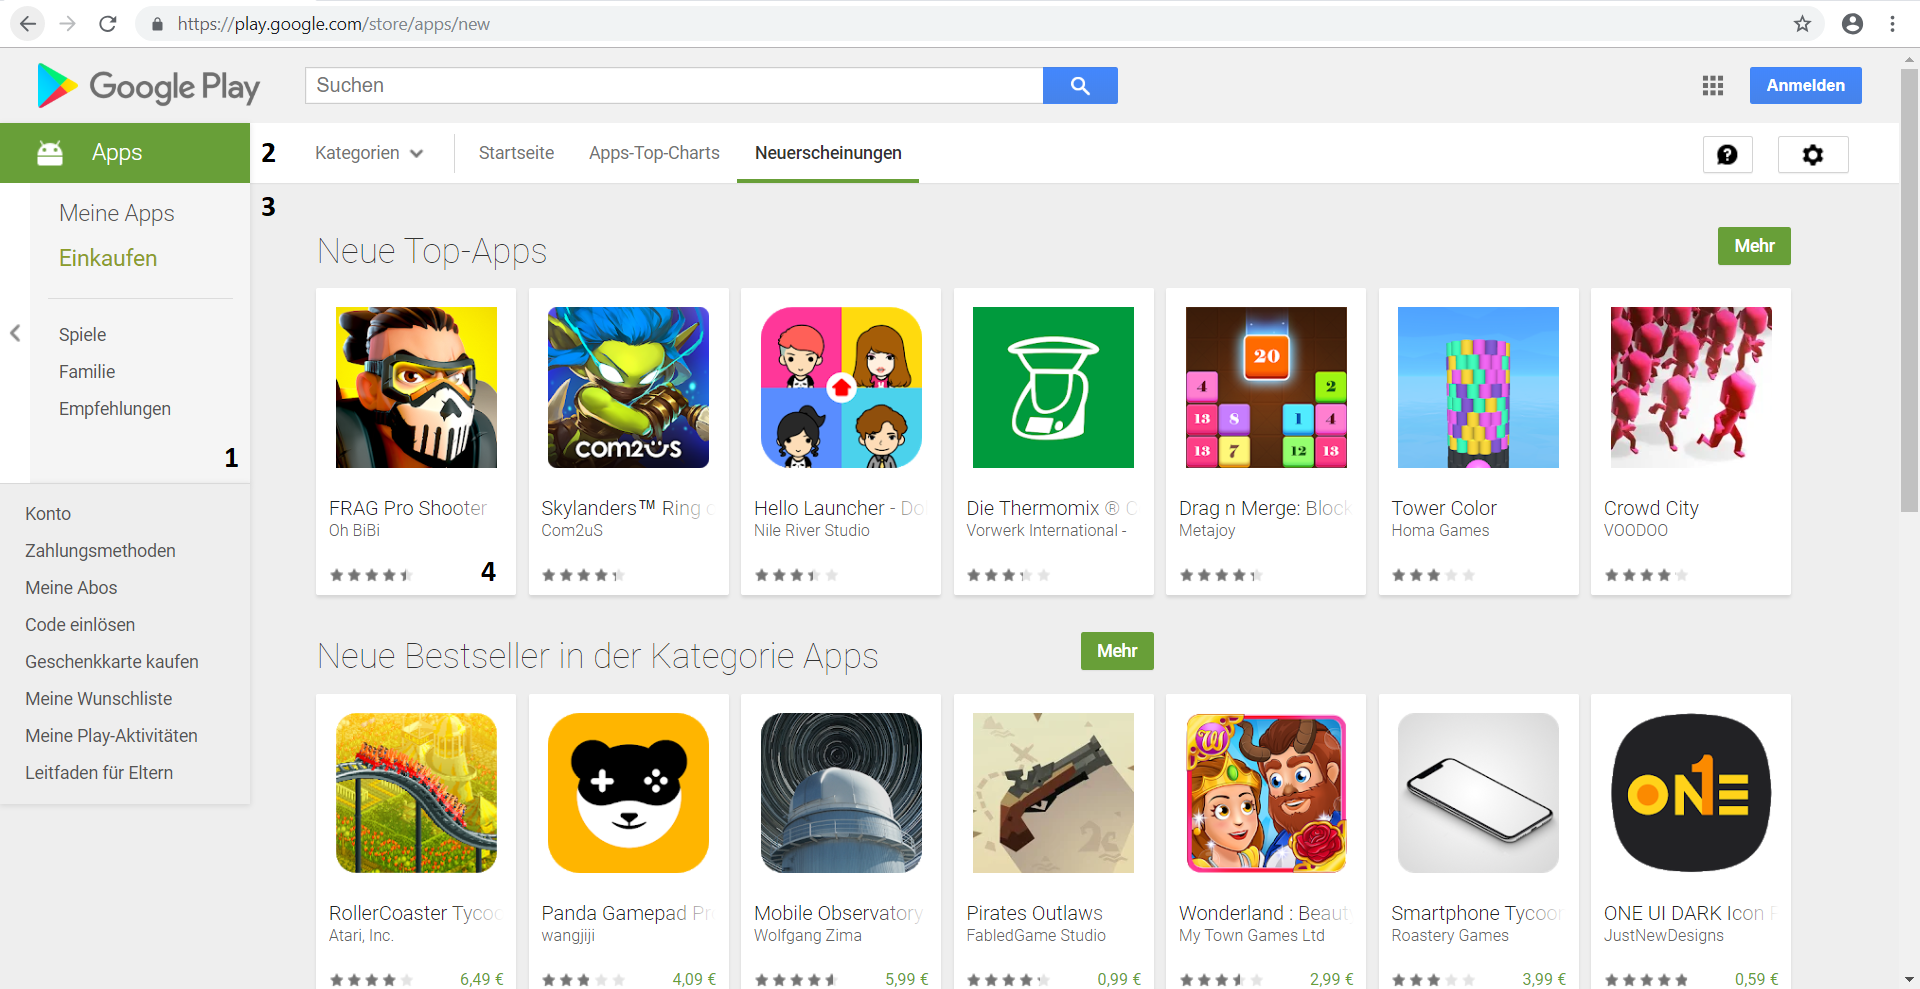
\includegraphics[width=1\textwidth]{pics/playstore1num.png}
	\caption{Kategorie Apps im Google Play Store (1: Apps-Menü; 2: Reiter; 3: Anzeigebereich der Apps; 4: Einzelne Kachel)}
	\label{playstore1}
\end{figure}

Alle Auswahlpunkte zeigen im Darstellungsbereich(Abb. \ref{playstore1} Nr.3) Apps in der gleichen Struktur an. Wie in Abbildung \ref{playstore1} zu erkennen, werden zu einer Thematik mehrere Kacheln(Abb. \ref{playstore1} Nr.4) in einer Reihe dargestellt. Durch den Button \glqq Mehr\grqq{} klappt die entsprechende Reihe aus. Aufgeklappte Themengebiete, Suchergebnisse und \glqq Meine Apps\grqq{} werden als Raster dargestellt.

Durch den Klick auf eine Kachel lädt der Nutzer die Detailseite(Abbildung \ref{playstore2}). Diese zeigt neben der ausgewählten App auch ähnliche Programme an der rechten Seite an. Auf der Basis aller hier gezeigten Informationen trifft der Nutzer die Entscheidung, ob die App installiert werden soll.

\begin{figure}[ht]
	\centering
	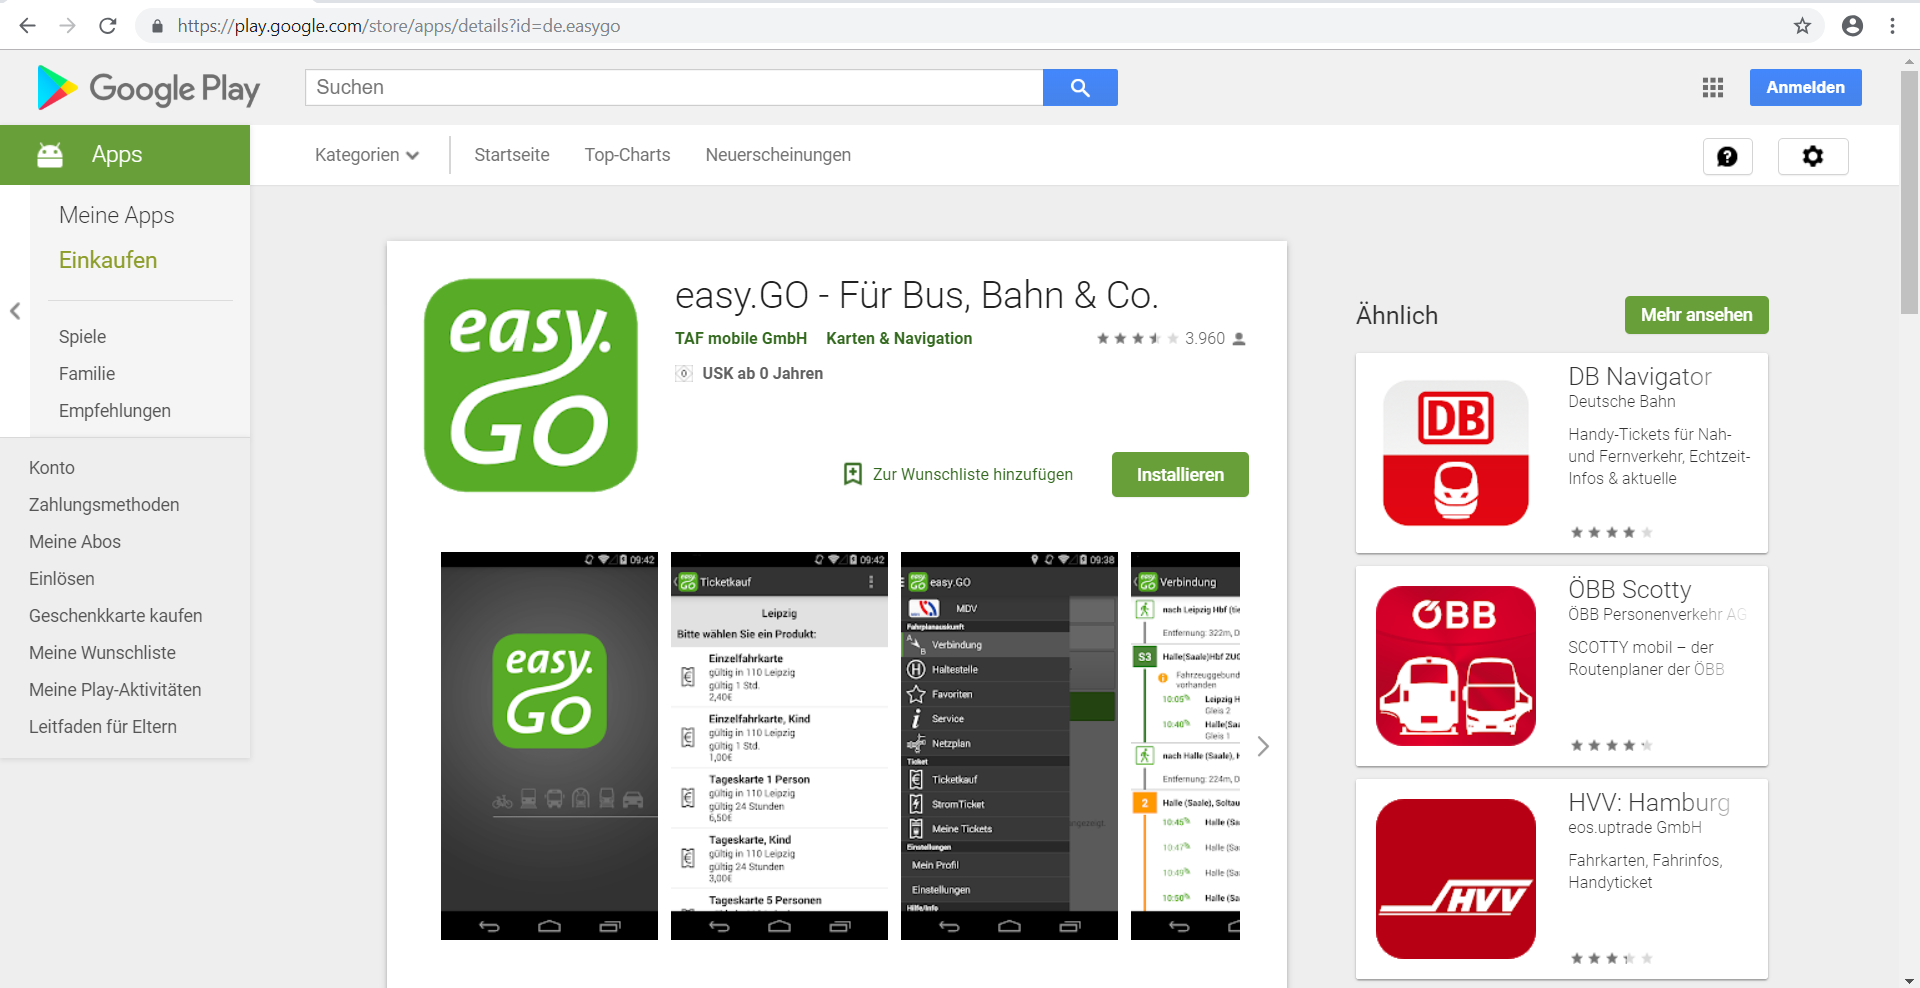
\includegraphics[width=1\textwidth]{pics/playstore2.png}
	\caption{Detailansicht einer App}
	\label{playstore2}
\end{figure}

Für die Funktionen der Erweiterung sind die Kacheln mit Informationen zu einzelnen Apps ausschlaggebend. Insgesamt unterscheidet die Website in drei Arten von Kacheln:

\begin{itemize}
	\item \textbf{Kleine Kachel}:	
	Wie in Abbildung \ref{playstore1} zu sehen, füllen kleine Kacheln alle Übersichtsseiten und sind als Reihe oder Raster angeordnet. Sie bestehen aus drei Bereichen. Das ist Vorschaubild oben, der Titel der App mit Herausgeber in der Mitte und die Bewertung unten zusammen mit dem Kaufpreis, falls vorhanden.
	
	\begin{figure}[ht]
		\centering
		
\includegraphics{pics/kachel1.png}
		\caption{Kleine Kachel}
		\label{kachel1}
	\end{figure}

	\item \textbf{Mittlere Kachel}:
	Als Raster unter dem Menü-Punkt \glqq Meine Apps\grqq{} und als vertikale Reihe neben einer großen Kachel in der Detailansicht(Abb. \ref{playstore2}) werden mittlere Kacheln eingesetzt. Diese, im Querformat dargestellte, Variante nimmt mehr Platz ein und bietet mehr Informationen.
	Das Vorschaubild ist links. In der rechten Hälfte oben befindet sich der Titel mit Herausgeber, darunter die Kurzbeschreibung der App. Am rechten unteren Rand sitzt die Bewertung mit dem Kaufpreis.
	
	\begin{figure}[ht]
		\centering
		
\includegraphics{pics/kachel2.png}
		\caption{Mittlere Kachel}
		\label{kachel2}
	\end{figure}

	\item \textbf{Große Kachel}:
	Jede App besitzt eine Detailansicht auf einer separaten Seite(Abb. \ref{playstore2}). Diese Details werden in der großen Kachel dargestellt.
	Der obere Teil ist nahezu identisch aufgebaut wie die mittlere Kachel. Darunter folgen Vorschaubilder, eine ausführliche Beschreibung, Nutzerbewertungen, der Updateverlauf und zusätzliche Informationen in Steckbriefform.
	\begin{figure}[ht]
		\centering
		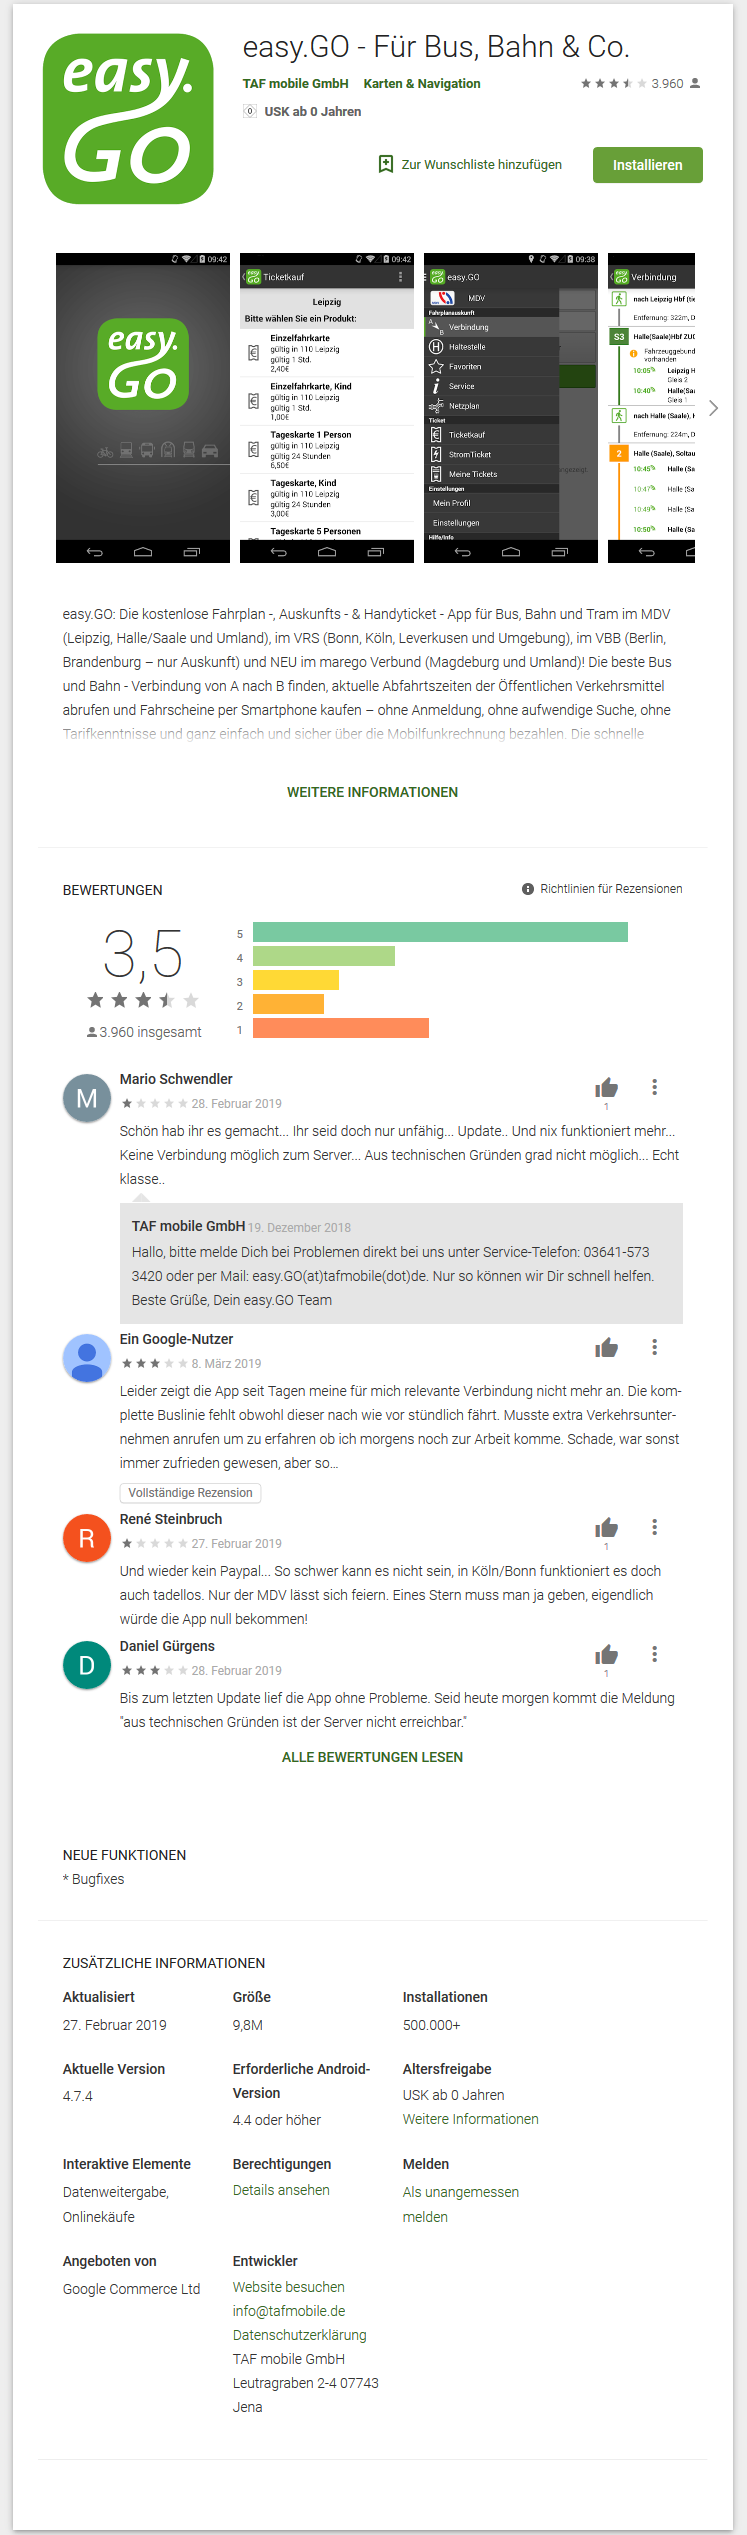
\includegraphics[scale=0.2]{pics/kachel3.png}
		\caption{Große Kachel}
		\label{kachel3}
	\end{figure}

\end{itemize}

Der in diesem Kapitel beschriebene Stand der Website bezieht sich auf den Zeitraum von März 2018 bis März 2019. Die Planung und Implementierung der Extension ist auf diesen optischen und technischen Stand der Website angepasst. Mögliche Probleme, die ein veränderter Stand der Website mit sich bringt, werden in Abschnitt \ref{ss:diskussionht1} diskutiert.

\subsection{Programmaufbau}
\label{ss:programmaufbau}
Die Implementierung des Programms orientiert sich an den beschriebenen Richtlinien in Kapitel~\ref{ss:funktionsumfang}. Dieser Abschnitt befasst sich mit der Umsetzung der Anforderungen aus Kapitel \ref{sss:funktionaleanforderungen}. Dabei werden relevante Ausschnitte des Quellcodes betrachtet und getroffene Entscheidungen begründet. Außerdem werden kritische Stellen beleuchtet und in Kapitel \ref{ss:diskussionht1} diskutiert.


\lstinputlisting[label={src:manifest}, caption={Aufbau der manifest.json}]{../../Extension/src/manifest.json}

Das Manifest stellt die grundlegenden Zusammenhänge der Extension dar. Unter anderem den gewählten Entwicklungsnamen der Extension \glqq PrivacyGuard App-Rating\grqq{} und die entsprechende Beschreibung.
Weiterhin sind die nötigen Berechtigungen aufgeführt:

\begin{itemize}
	\item \textbf{storage}:
	Berechtigung zum Zugriff auf Speicherplatz, um Informationen aus Backend-Anfragen zu speichern. Details zu konkreten Möglichkeiten der Speicherplatznutzung behandelt Kapitel~\ref{ss:anforderungen}.
	\item \textbf{declarativeContent}:
	Bereitstellung von Events, wie Seitenaufruf oder -änderung und damit zusammenhängende Regeln, wie das Ausführen von Content-Skripten. Diese API wird vom Background-Skript genutzt,welches die genannten Aufgaben umsetzt.
	\item \textbf{activeTab} und \textbf{tab}:
	Gibt an, ob sich der Nutzer gerade in einem Tab befindet auf dem die Extension aktiv ist.
\end{itemize}

Außerdem werden alle Dateien ihren Rollen zugewiesen:

\begin{itemize}
	\item \textbf{Content-Skript}:
	Unter dem Punkte \glqq content scripts \grqq{} wird festgelegt, welche Skripte unter welchem URL aktiv sind.
	
	Der Ausdruck \glqq *://play.google.com/store/apps*\grqq{}
	bedeutet, dass die Extension auf jeder Playstore-Seite der Kategorie Apps und deren Unterverzeichnis aktiv ist. Da es sich um eine \glqq page action\grqq{} Extension handelt, wird lediglich eine Website als \glqq match \grqq{} aufgeführt. Die beiden wichtigen Dateien hier sind \glqq pguard.js\grqq{} als das Content-Skript für sämtliche Funktionen die die Erweiterung der Website betreffen und \glqq popup-controller.js\grqq{} für alle Funktionen des Popups. Hinzu kommen sämtliche Bibliotheken, welche von den Content-Skripten benötigt werden.
	
	\item \textbf{Background-Skript}:
	Das Background-Skript \glqq background.js\grqq{} fungiert als Eventhandler der Extension ist deshalb separat im Manifest aufgeführt.
	
	\item \textbf{web\_accessible\_resources}:
	Diese Ressourcen sind Dateien welche der Extension zur Verfügung stehen, aber selber keine Skripte sind. Sie beinhalten ausgelagerte Informationen wie Fließtexte und Templates zum Bauen von HTML-Elementen. Die \glqq popup.html\grqq{} ist hier ein Sonderfall und wird direkt dem Popup zugewiesen.
\end{itemize}

Die Background.js besteht lediglich aus Callback-Funktionen der declarativeContent API. Hier wird zur Installation der Extension ein Listener eingebunden. Dieser funktioniert mit Regeln nach dem Konditionen-Aktionen-Prinzip. Zum Start des Aufrufs werden alle bereits vorhandenen Regeln des Listeners entfernt und anschließend die übergebenen Regeln installiert.
Hier benötigt das Programm eine Regel. Die Kondition prüft ob der passende URL aufgerufen wurde. Dieser stimmt mit dem String aus der Manifest-Datei überein. Ist die Kondition erfüllt, aktiviert sich das Popup.


\lstinputlisting[label={src:background}, caption={background.js}]{../../Extension/src/background.js}

Das Content-Skript pguard.js bildet den Hauptteil der Extension und dient zur Erfassung aller, auf der Webseite dargestellten Apps, der Einbettung von zusätzlichen Informationen durch das PGuard-Backend und optischen Anpassung der Webseite, um die neuen Inhalte ordentlich einzubinden.

Bei Skript-Aufruf werden zuerst die lokalen Bibliotheken der Extension geladen. Dazu gehören die IB texte.json sowie die HTML-Templates. Außerdem überprüft das Skript, ob lokaler Speicher zur Verfügung steht.

Anschließend prüft die Funktion \glqq fillApps\grqq{}, ob die aktuelle Seite eine Single-App-Page oder Mutli-App-Page ist und ermittelt sämtliche Kandidaten, welche für die Einbettung der Informationen in Frage kommen. Dabei liest der JQuery-Selektor alle Elemente mit dem entsprechenden Klassnamen aus.

Mit der Funktion \glqq loadInfoPanels\grqq{} wird jeder so gefundene Kandidat auf seine APP-ID überprüft. Diese befindet sich entweder in dem Attribut \glqq data-docid\grqq{} oder \glqq href\grqq{}. Mithilfe dieser ID durchsucht die Funktion \glqq getStorageItem\grqq{} den lokalen Speicher auf Einträge. Der  Eintrag ist valide, falls er nicht leer ist und vor weniger als 3 Tagen angelegt wurde. Findet die Funktion keinen validen Eintrag im lokalen Speicher, wird eine neue Anfrage an das Backend, für die entsprechende APP-ID, erstellt.

%BEISPIEL ANFRAGE

Liefert das Backend eine Antwort mit mindestens einem Ergebnis, speichert die Funktion die Informationen im lokalen Speicher ab. Bei mehr als einem Ergebnis, entscheidet eine Prioritätenliste abhängig von der zuverlässigsten Quelle, welcher Datensatz genutzt wird.

Der gewählte Datensatz wird der Funktion \glqq createPanel\grqq{} übergeben. Handelt es sich bei dem Kandidaten um eine App-Page(Single-App), wird das Popover aus den Informationen direkt erstellt. Dazu wird der Datensatz mit Hilfe der IB texte.json in den entsprechenden Text umgewandelt und in die Html-Template einfügt.
Bei kleinen App-Kacheln baut die Funktion einen Banner in die Kachel ein. Auf diesem Banner wird mittels JQuery ein Event geladen, welches bei einem Klick auf den Banner das Popover erstellt.

\begin{figure}[ht]
	\centering
	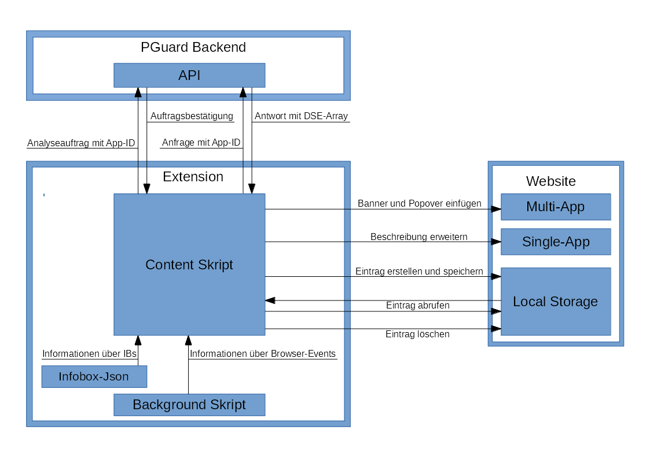
\includegraphics[width=1\textwidth]{pics/Aufbau.png}
	\caption{Aufbau und Interaktionen der Extension}
	\label{aufbau}
\end{figure}


\subsection{Ergebnis}
\label{ss:ergebnisseht1}

Die Browser-Extension stellt Datenschutzinformationen an mehreren Stellen der Webseite zur Verfügung. Bei kleinen und mittelgroßen Kacheln wird der erstellte Banner mit der Anzahl an gefundenen Infoboxen am oberen Rand eingeblendet (siehe Abbildung \ref{ergebnis1}). Die Darstellung unterscheidet sich dabei je nach Status der Informationen:

\begin{itemize}
	\item \textbf{\glqq Keine Ergebnisse\grqq{}}:
	Aufgrund von technischen Problemen liefert das Backend keine Datenschutzinformationen zu der angefragten Applikation.
	\item \textbf{Blauer Banner}:
	Informationen zum Datenschutz über die Applikation sind vorhanden, aber es liegt kein möglicher Gesetzesverstoß oder erheblicher Nachteil für den Nutzer vor.
	\item \textbf{Roter Banner (\glqq Rote Linie\grqq{})}:
	Informationen zum Datenschutz über die Applikation sind vorhanden und es liegt ein möglicher Gesetzesverstoß, bzw. ein erheblicher Nachteil für den Nutzer vor.
\end{itemize}

\begin{figure}[ht]
	\centering
	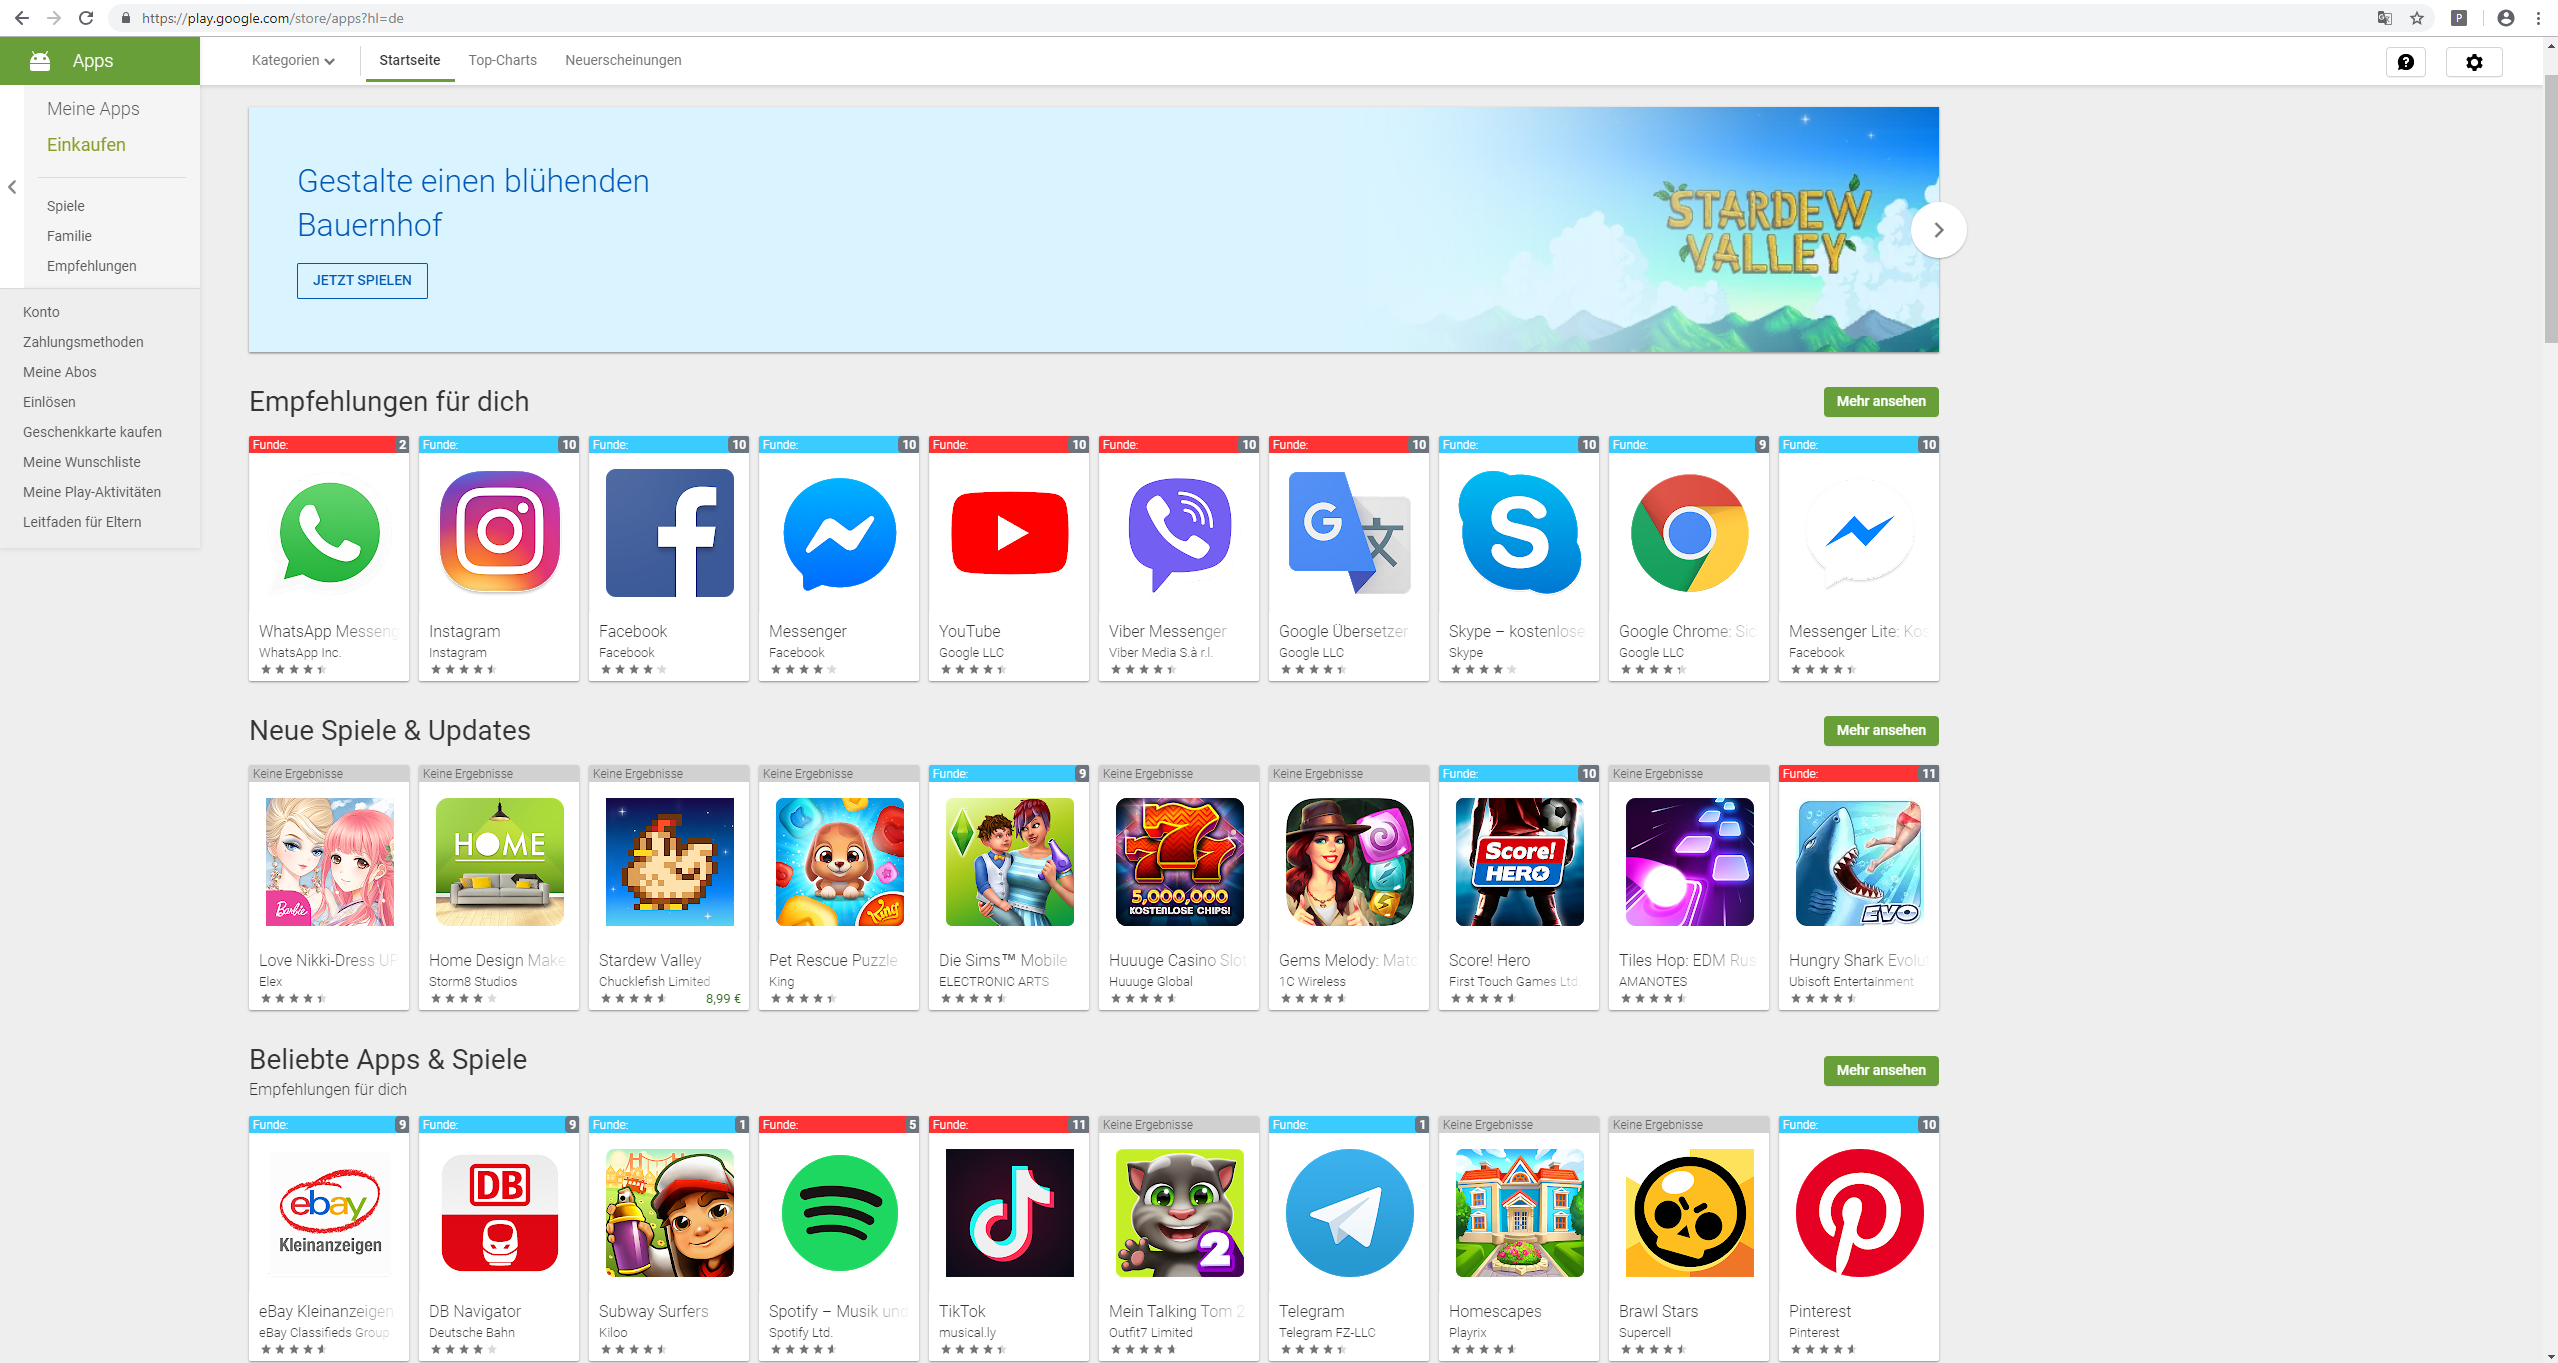
\includegraphics[width=1\textwidth]{pics/ergebnis1.png}
	\caption{Ergänzung der Kacheln durch farbige Banner.}
	\label{ergebnis1}
\end{figure}

Durch einen Klick auf den Banner erscheint das jeweilige Popover, bestehend aus einem Fenster mit der Liste an gefundenen Infoboxen. Diese Boxen sind aufklappbar und beinhalten die jeweilige Beschreibung, Handlungsempfehlungen, Vor- und Nachteile.

\begin{figure}[ht]
	\centering
	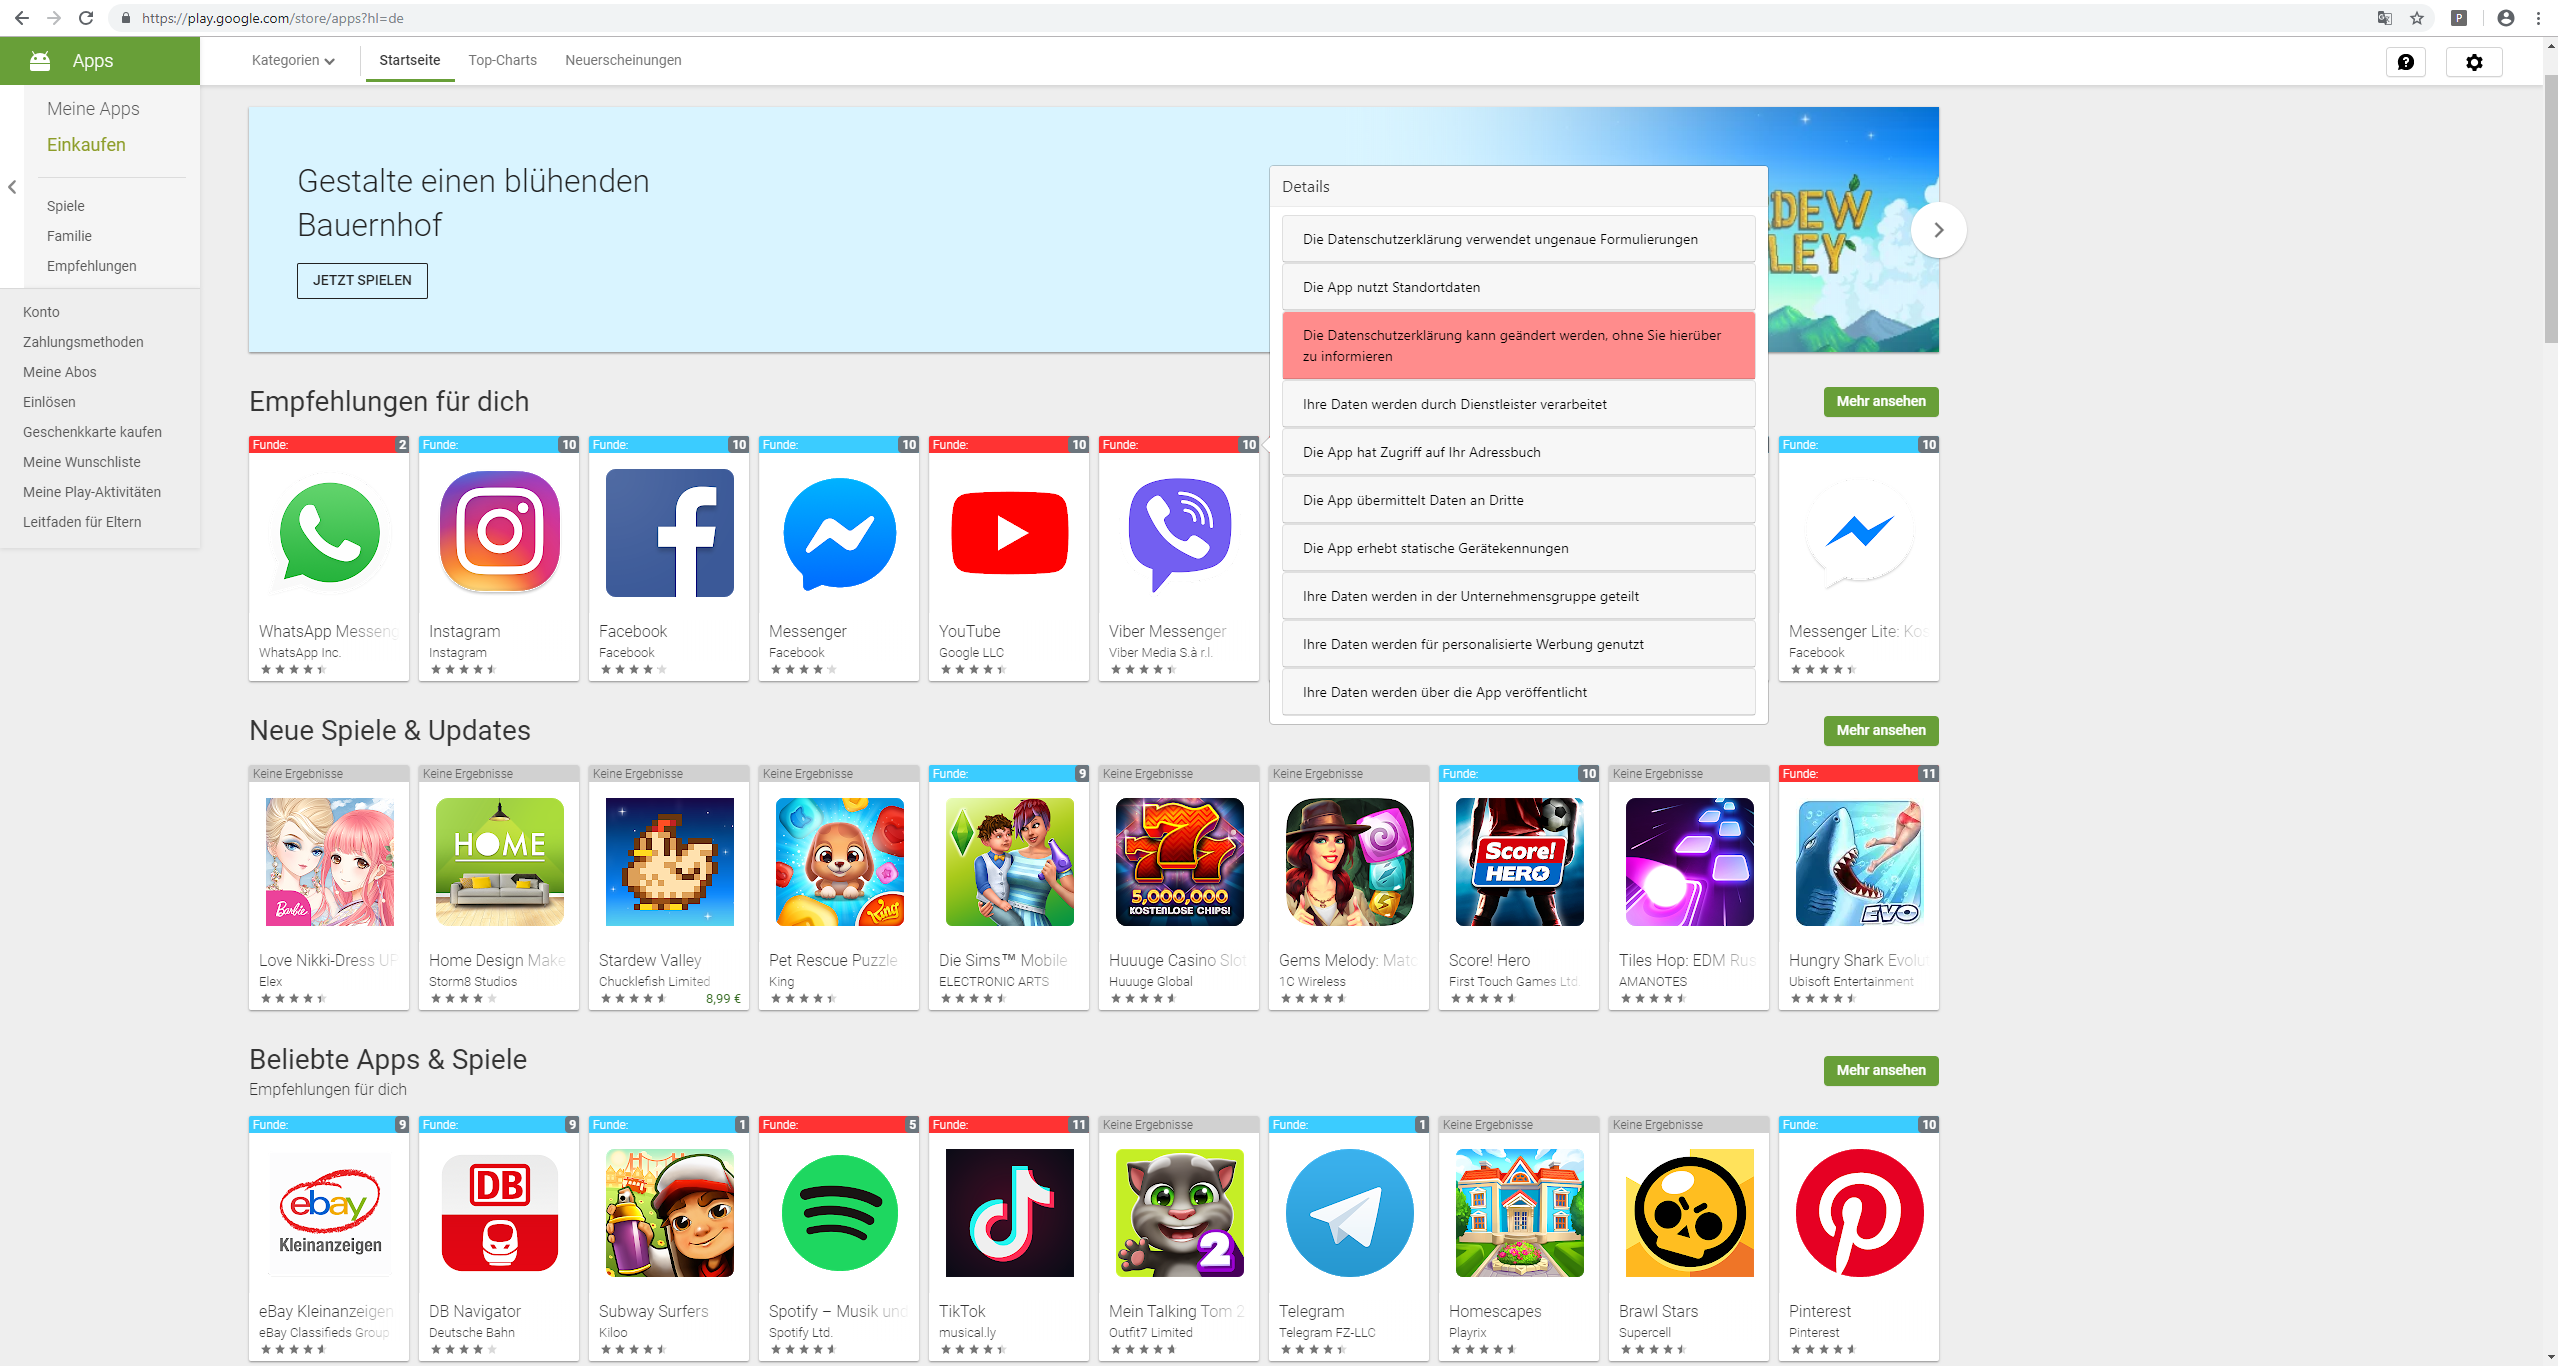
\includegraphics[width=1\textwidth]{pics/ergebnis2.png}
	\caption{Popover mit der Auflistung an Infoboxen. \glqq rote Linien \grqq{} sind entsprechend markiert.}
	\label{ergebnis2}
\end{figure}

Auf den Detailseiten wird dieses Fenster direkt in die große Kachel, zwischen der Programmbeschreibung und den Bewertungen eingebettet. Die Templates sind hier identisch zu denen im Popover.

\begin{figure}[ht]
	\centering
	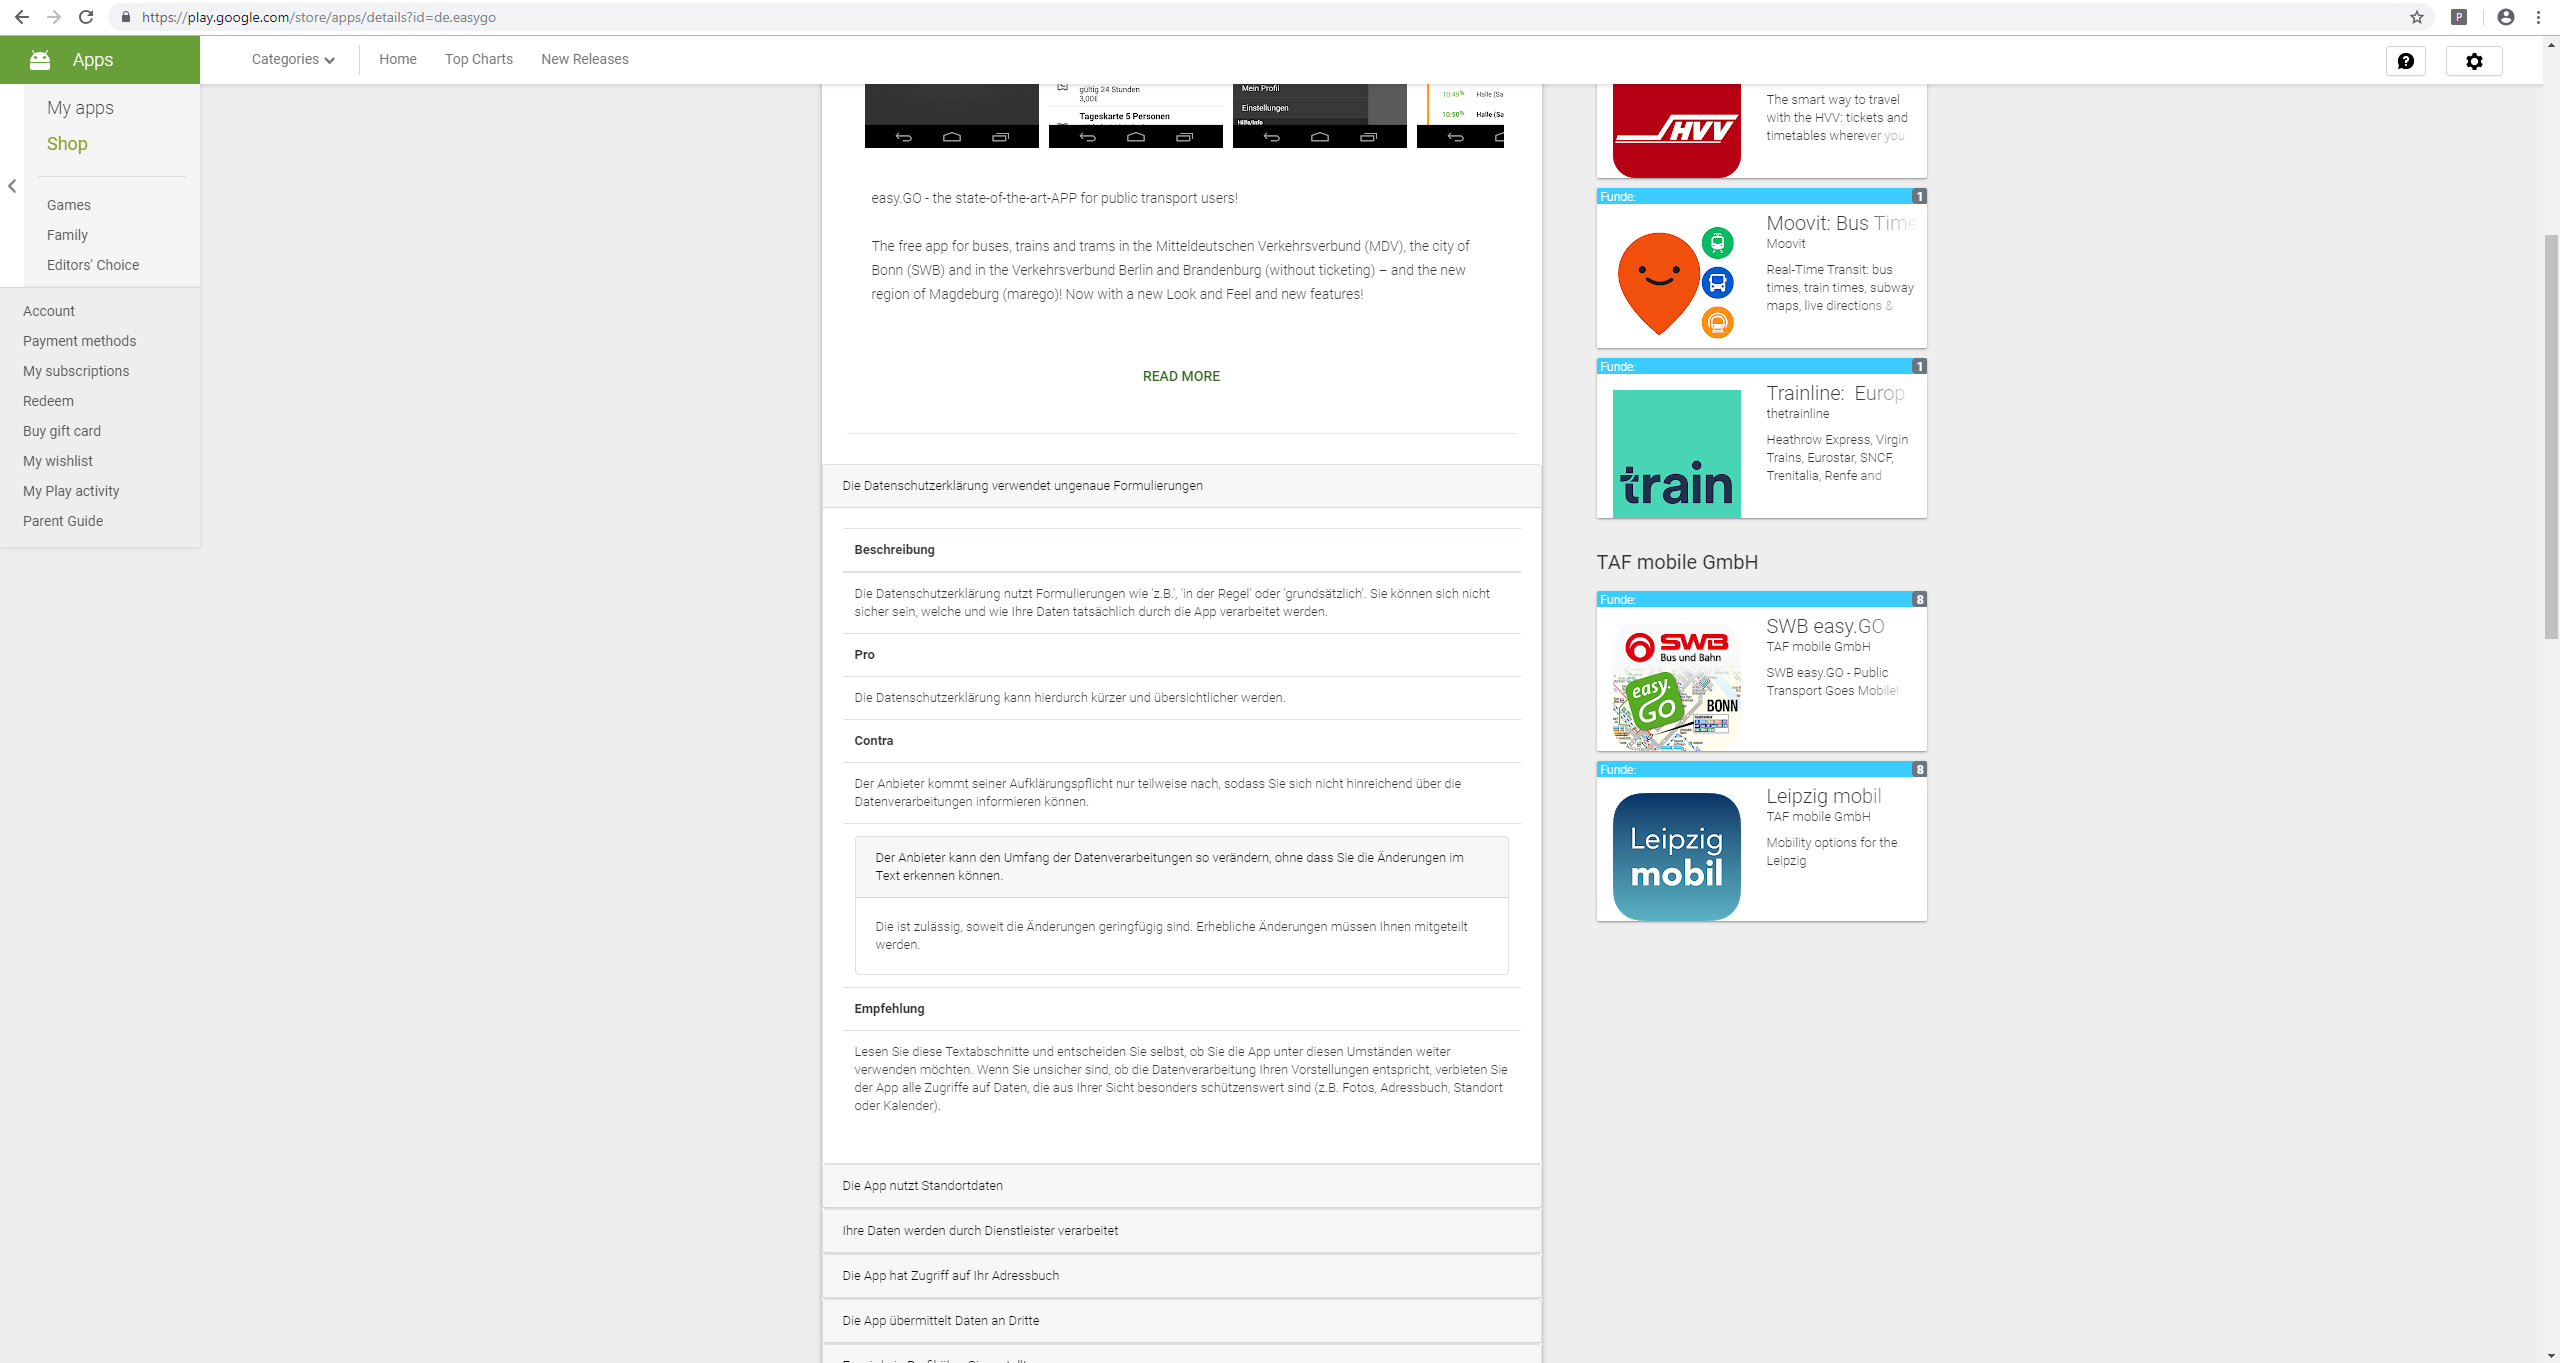
\includegraphics[width=1\textwidth]{pics/ergebnis4.png}
	\caption{Detailseite mit eingefügten Infoboxen.}
	\label{ergebnis4}
\end{figure}

Alle, vom Backend gewonnenen, Informationen werden in eine lokale Datenbank abgespeichert und beim nächsten Auftauchen der gleichen Kachel wieder ausgelesen. Nach drei Tagen gilt die Information als veraltet und wird auf Abruf aktualisiert. Kapitel \ref{ss:anforderungen} befasst sich mit dem genauen Aufbau der Datenbank.

Das Icon besitzt ein Popup-Menü mit zwei Buttons zum Aktivieren/Deaktivieren der Extension und zum Löschen der angelegten Datenbank.

\subsection{Diskussion}
\label{ss:diskussionht1}

Im Verlauf der Programmierung sind technische und organisatorische Probleme aufgetreten. Hier werden einige davon erläutert und deren Konsequenzen aufgezeigt.

Da sich diese Browser-Extension sehr an der aktuellen Struktur der Website orientiert, können in Zukunft Fehler bei der Darstellung der Banner und Templates auf der Seite auftreten. Während der Implementierung traten bereits einige dieser Fehler auf.

Der Klick, welcher das Event zum Auf- und Zuklappen der Infoboxen auslöst, überlappt sich mit anderen Events der Webseite, auf die die Extension keinen Einfluss hat. Generell erschwert die Undurchsichtigkeit des technischen Aufbaus der Website die Anpassung der Funktionen einer Extension. Sodass bei der Implementierung das Testen aller eingefügten Elemente manuell geschieht und mit großen Mehraufwand verbunden ist.

Weiterhin überarbeitet Google die Website in regelmäßigen Abständen. Die in dieser Arbeit getroffene Aufteilung in Kacheln kann mit der nächsten Überarbeitung bereits obsolet sein. Aufgefallen ist das bei Betrachtung der Website in den letzten Monaten. Dabei haben sich bereits einige Klassennamen von Elementen der Kacheln geändert, sodass die Banner in falscher Größe oder gar nicht dargestellt worden.

Im Allgemeinen ist die Browser-Extension in ihrem aktuellen Zustand nicht \glqq marktreif \grqq{}. Das heißt, es Bedarf weiterer Überarbeitung und Organisation bevor man die Extension im Web-Store von Google anbieten kann. 

Aufgrund der Evaluation von möglichen lokalen Datenspeichern für diese Extension, sind sowohl \glqq IndexedDB\grqq{} als auch \glqq LokalStorage\grqq{} implementiert. Für spätere Verbraucher müsste eine der beiden Methoden entfernt werden, um unnötige Verwirrung im Umgang mit der Extension zu vermeiden.

Bereits in der Implementierungsphase sind inkonsistente Datensätze aufgefallen.Eine genauere Überprüfung ergab, dass die automatisierte Informationsgewinnung und Verarbeitung teilweise fehlerhaft ist. Dazu zählen das Crawlen von Datenschutzerklärungen aus unzuverlässigen Quellen und das priorisieren der falschen Sprache. Dadurch kann die Richtigkeit der anzeigten Informationen nicht vollumfänglich garantiert werden. Auf dieser Basis wäre eine Funktion zur Empfehlung von alternativen Apps nicht sinnvoll.

Das Forschungsprojekt PrivacyGuard wurde im Juni 2018 beendet und somit auch die Verwaltung aller, in diesen Rahmen entstandenen, Produkte. Deshalb gibt es zum aktuellen Zeitpunkt keinen Verantwortlichen für die Veröffentlichung und Wartung des Backends und dieser Extension.